% vim:ts=4:sw=4
% Copyright (c) 2014 Casper Ti. Vector
% Public domain.

\chapter{系统实现}
\section{爬虫模块}
基于在本文第二部分中的数据来源和爬虫的分析,采用beautifulSoup技术来进行扒取数据。
\subsection{爬取基本数据}
\begin{figure}[h]
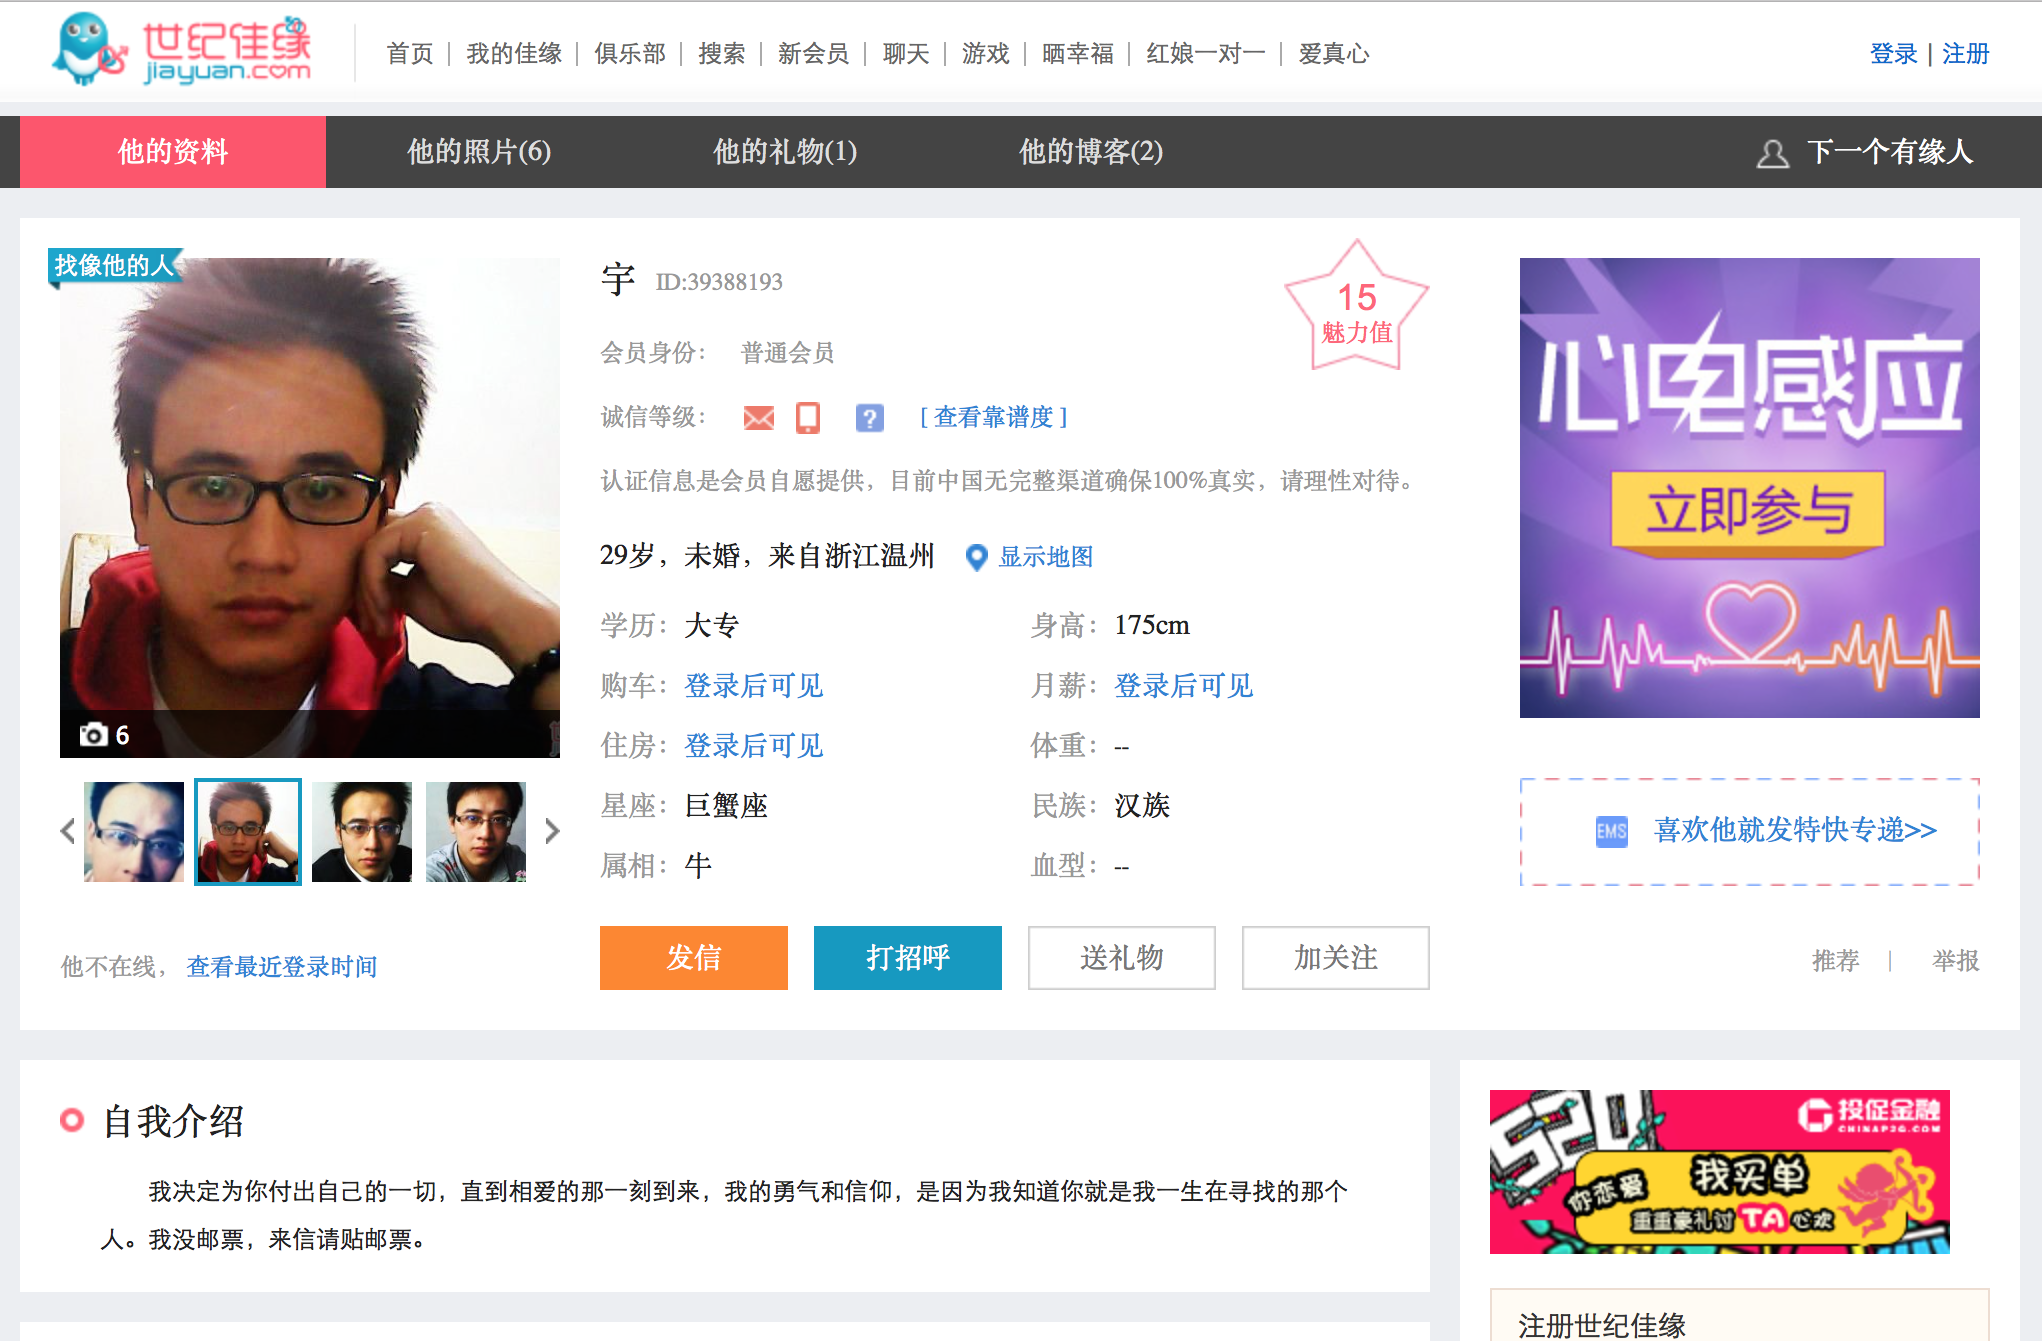
\includegraphics[width=\textwidth]{img/chap4/jiayuan1.png}
\caption{世纪佳缘用户信息页面\label{Face++API}}
\end{figure}
\begin{figure}[h]
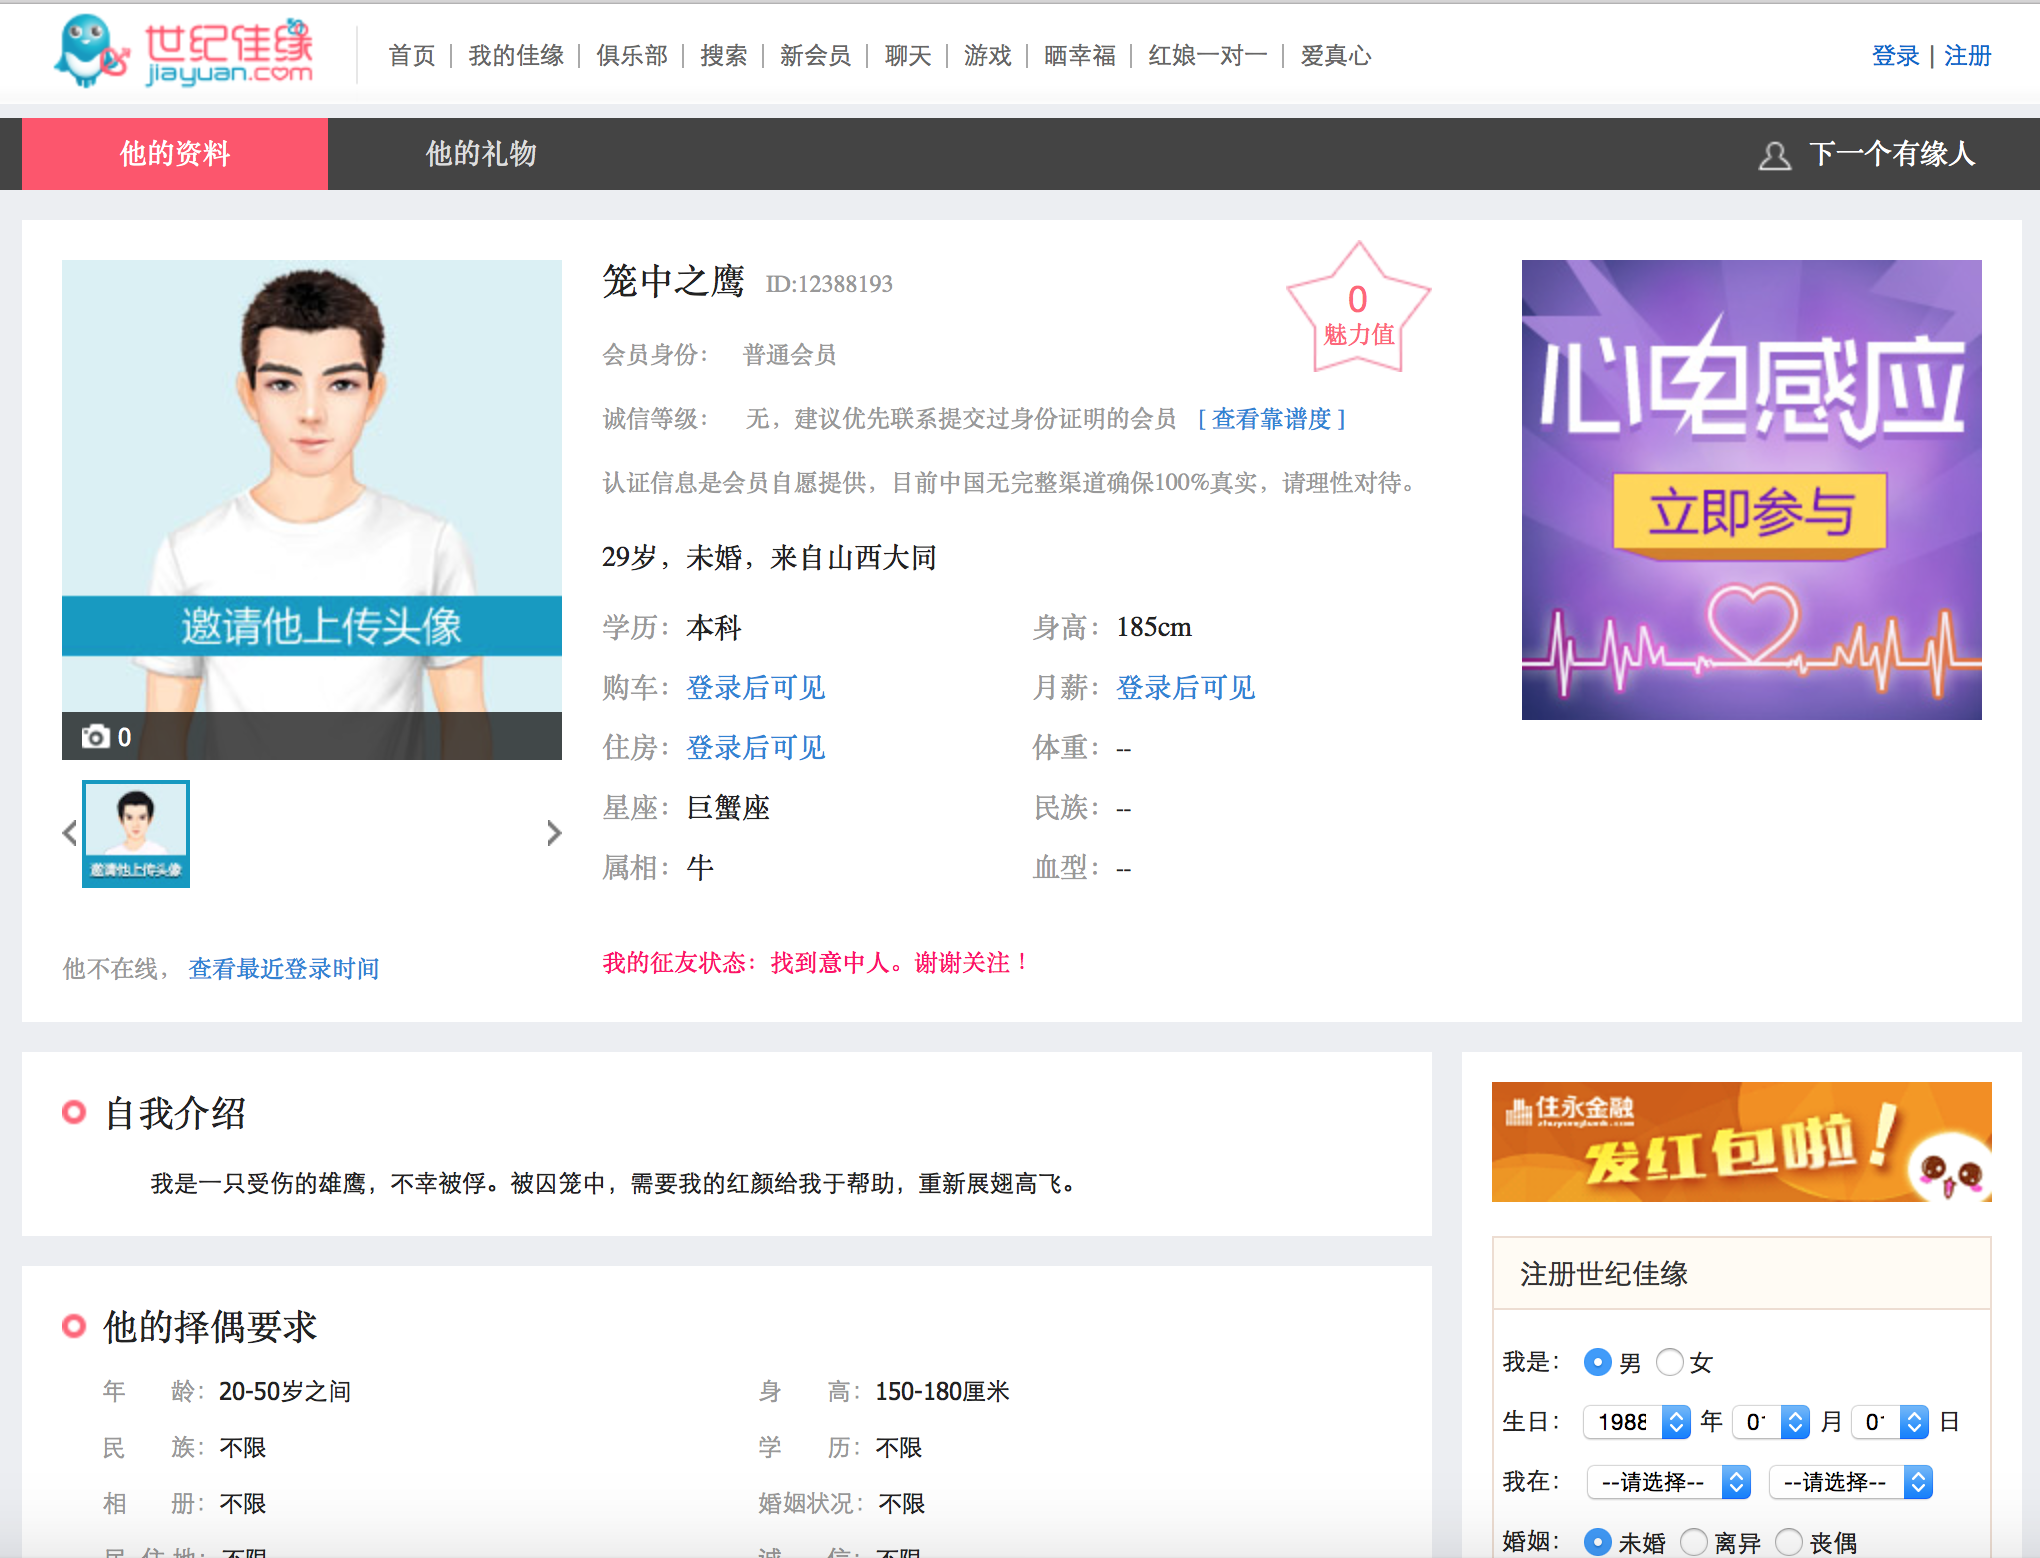
\includegraphics[width=\textwidth]{img/chap4/jiayuan2.png}
\caption{世纪佳缘需权限信息页面\label{Face++API}}
\end{figure}

通过前期充分对于世纪佳缘网站上数据的发掘,本文找到了一个基于用户id以及对应用户数据的网页,从图4.1,图4.2可以看出,此网页url为用户id与前缀结合,而除了一些用户的图片和信息设置为成权限可见之外,其他的数据对于爬虫都是友好的。

[伪代码1]
\subsection{导入数据库}
提交到用户数据库的代码
[伪代码2]

\section{应用端模块}
该应用的实现由三步组成:状态查询,信息源添加,和匹配反馈。
具体的应用端的逻辑,由一个类似的iOS框架图来类比。

\subsection{状态查询及展示}
用户在使⽤应⽤程序查看他人已经存在的用户信息,需进行对于用户信息的一个预览,以及对于具体应用信息的查询。

根据用户需求可以查看具体的信息,并可以支持用户随时对于需要的信息的刷新,以及链接用户更进一步的个人主页的途径。
针对
[伪代码2][贴实际效果图]
\subsection{信息源添加}
信息发布者在使⽤用应⽤用程序添加信息源时,需进⾏行上下⽂文采集和添加详细信息 两⽅方⾯面操作。
由于前⽂文提到的传感器数据在精确度和稳定性上的弊端,为了改善整个系统的 ⼯工作效果,上下⽂文采集过程需要在应⽤用程序⾃自动采集传感器数据的基础上,增加⼀一 定的⼈人⼯工⼲干预以进⾏行优化。对于位置信息,应⽤用程序将采集到的坐标显⽰示为地图上 的⼀一个⼤大头针,如果⽤用户认为此位置不准确,可以拖动地图以调整到准确的位置。 对于磁场计信息和 iBeacon 信号,由于它们总是随着时间不停地变动,应⽤用程序将 它们以友好的形式显⽰示出来 (磁场计信息显⽰示为设备⽅方向⾓角度,iBeacon 信号显⽰示为 每个 iBeacon 的 minor identifi゙er 和距离值),⽤用户可以随时观察这些数值的变化,并 冻结在⽐比较满意的数值上 (图 1-a)。

信息发布者通常希望其发布的信息具有多种多样的形式,考虑到移动设备较难 编辑和显⽰示富⽂文本信息,应⽤用程序被实现为能够编辑、存储和显⽰示具有多种类型的 字段,包括标题、详细介绍、URL 或应⽤用程序跳转链接*和图⽚片 (图 1-b)。

基于用户照片来源的不同
[伪代码][实际效果图]
\subsection{匹配信息展⽰}
由于服务端将客户端提交的图片以及文本信息直接调用对应匹配算法的接口,因此, ⽤用户在选择了信息识别编码后,服务端便具有了⾜足够的信息以匹配出⽤用户想要了解 的信息源。在服务端返回给客户端匹配出的结果后,客户端将详细信息显⽰示在⽤用户 界⾯面上 (图3)。如果具有多条匹配结果,客户端将按照匹配程度顺序将结果显⽰示为列 表的形式。
[伪代码][实际效果图]
\subsection{详细资料界面}
[伪代码][实际效果图]


\section{}




% 中文测试文字。


